\documentclass{article}
\usepackage{graphicx}
\usepackage{hyperref}
\usepackage{float}

\title{libasm sources}
\author{Sadettin Fidan}
\date{\today}

\begin{document}

\maketitle

\section{Introduction}
I have implemented a library in assembly language. The resources I used will be mentioned and presented in this document.

\section{Functions in the library:}
\begin{itemize}
    \item ft\_strlen (man 3 strlen)
    \item ft\_strcpy (man 3 strcpy)
    \item ft\_strcmp (man 3 strcmp)
    \item ft\_write (man 2 write)
    \item ft\_read (man 2 read)
    \item ft\_strdup (man 3 strdup, you can call to malloc)
\end{itemize}

\section{Bonus Functions in the library}

\begin{figure}[H]
    \centering
    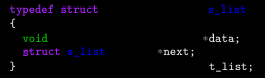
\includegraphics[width=0.4\textwidth]{struct_list.png}
    \caption{Struct list}
    \label{fig:struct_list}
\end{figure}

\begin{itemize}
    \item ft\_atoi\_base (like the one in the piscine)
    \item ft\_list\_push\_front (like the one in the piscine)
    \item ft\_list\_size (like the one in the piscine)
    \item ft\_list\_sort (like the one in the piscine)
    \item ft\_list\_remove\_if (like the one in the piscine)
\end{itemize}

\pagebreak

\section{Resources}

\subsection{General purpose Registers for Intel}

\begin{figure}[H]
    \centering
    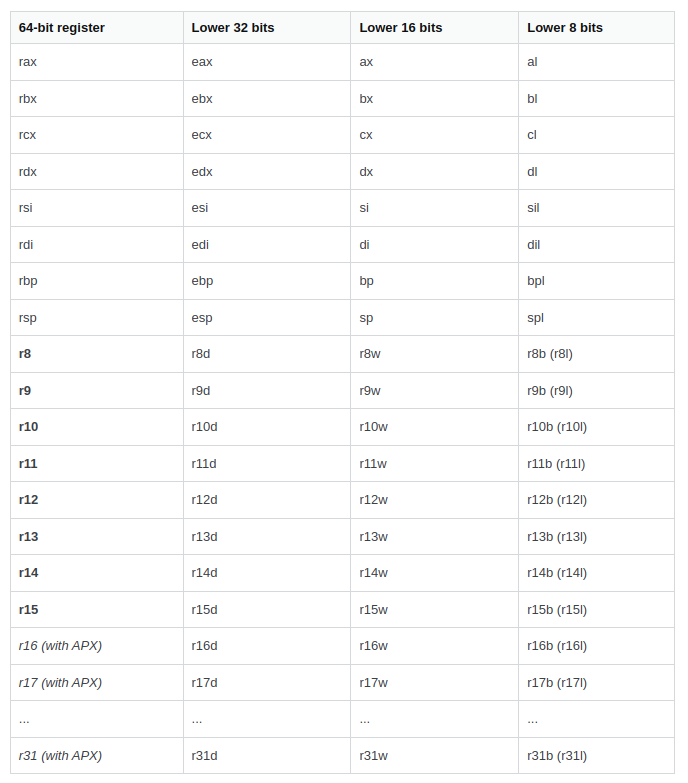
\includegraphics[width=\textwidth]{registers.png}
    \caption{General purpose Registers for Intel}
    \label{fig:registers}
\end{figure}

You can find the image in \ref{fig:registers} at: \url{https://stackoverflow.com/questions/20637569/assembly-registers-in-64-bit-architecture}

\subsection{Virtual Memory}

\begin{figure}[H]
    \centering
    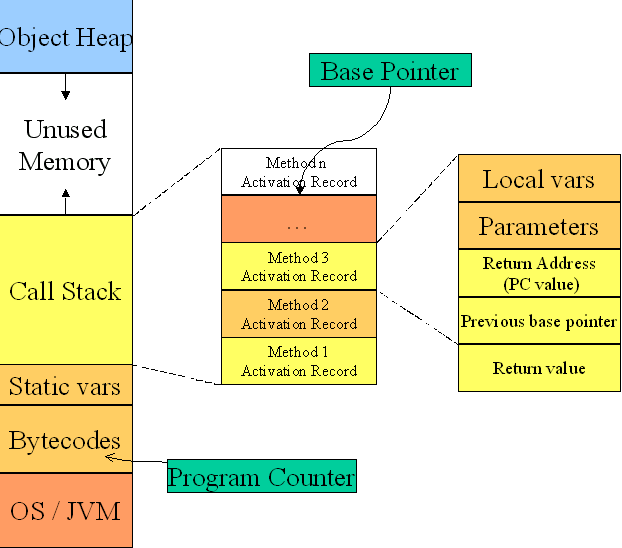
\includegraphics[width=\textwidth]{vm.png}
    \caption{Virtual Memory}
    \label{fig:vm}
\end{figure}

Using the figure \ref{fig:vm} as a reference, I used local variables inside functions. I get it from \url{https://learn.microsoft.com/en-us/cpp/build/stack-usage?view=msvc-170}

\subsection{x64 Intel Stack}

\begin{figure}[H]
    \centering
    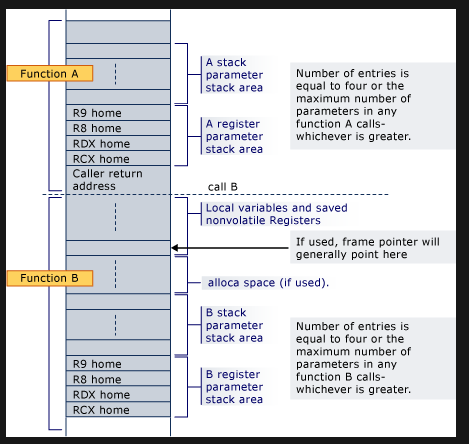
\includegraphics[width=\textwidth]{x64_stack.png}
    \caption{Stack in x64 Intel, as Function A and B}
    \label{fig:x64_stack}
\end{figure}

I used the figure \ref{fig:x64_stack} as a reference for the stack in x64 Intel. I get it from \url{https://en.wikipedia.org/wiki/X86_calling_conventions}

\subsection{System Calls}

\begin{figure}[H]
    \centering
    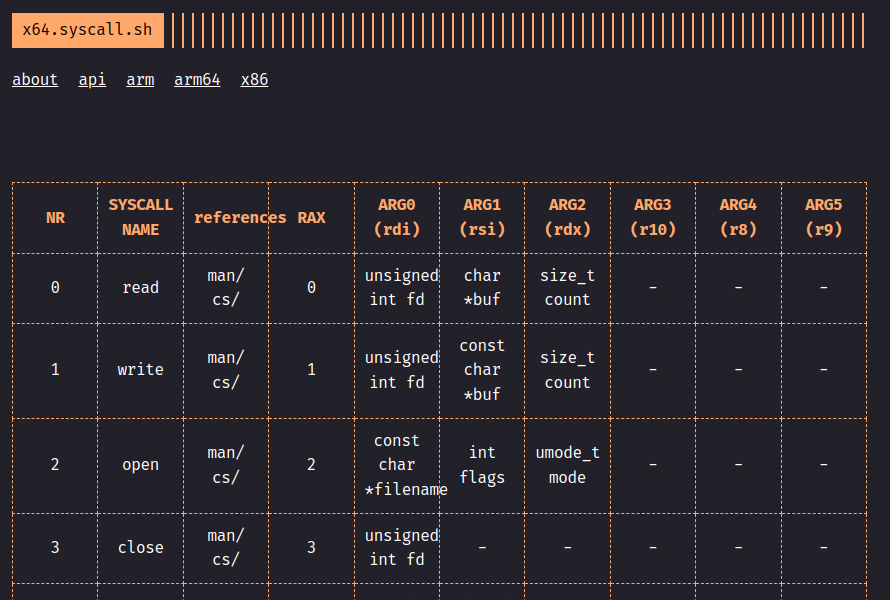
\includegraphics[width=\textwidth]{syscalls.png}
    \caption{System Calls}
    \label{fig:syscalls}
\end{figure}

I used the figure \ref{fig:syscalls} as a reference for system calls. I get it from \url{https://x64.syscall.sh/}

\subsection{Calling Convention}

\begin{figure}[H]
    \centering
    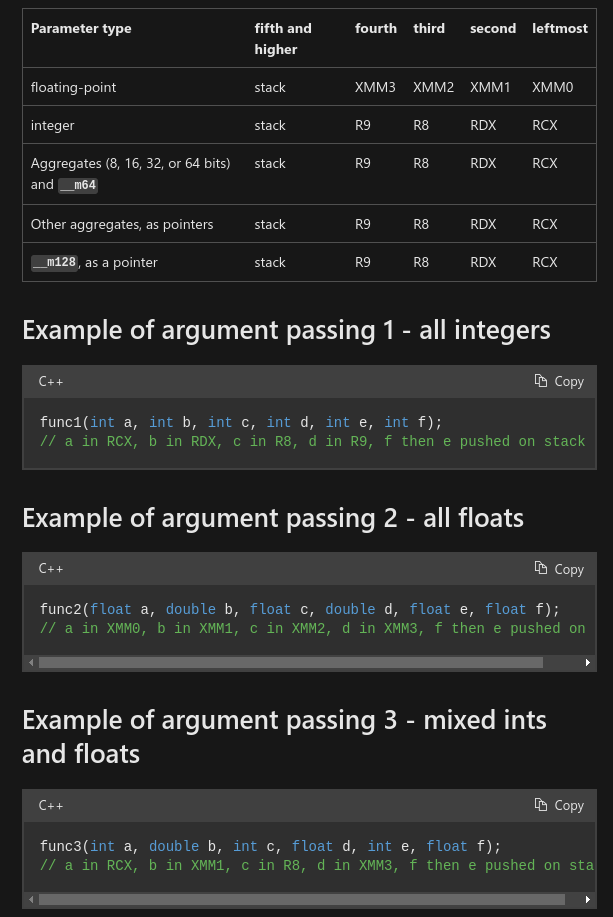
\includegraphics[width=0.7\textwidth]{calling_convention.png}
    \caption{x64 Intel calling convention}
    \label{fig:calling_convention}
\end{figure}

I used the figure \ref{fig:calling_convention} as a reference for calling convention. I get it from \url{https://learn.microsoft.com/en-us/cpp/build/x64-calling-convention?view=msvc-170}

\subsection{Assembly Code}

\begin{figure}[H]
    \centering
    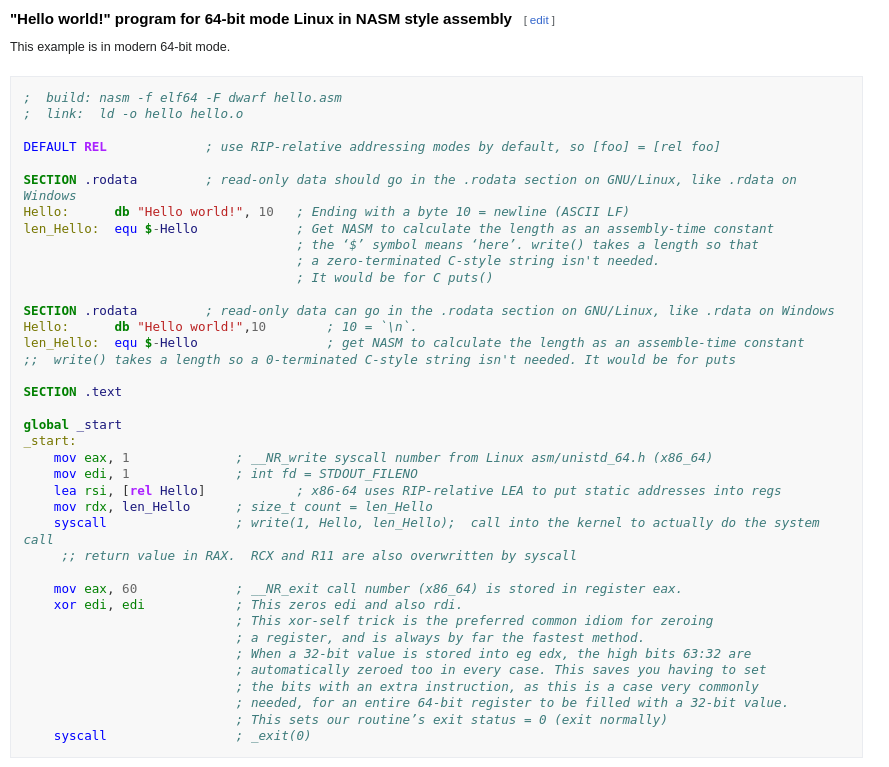
\includegraphics[width=\textwidth]{assembly_code.png}
    \caption{Assembly Code}
    \label{fig:assembly_code}
\end{figure}

I used the figure \ref{fig:assembly_code} as a reference for assembly code. I get it from \url{https://en.wikipedia.org/wiki/X86_assembly_language}

\subsection{Debugging with GDB}

\begin{figure}[H]
    \centering
    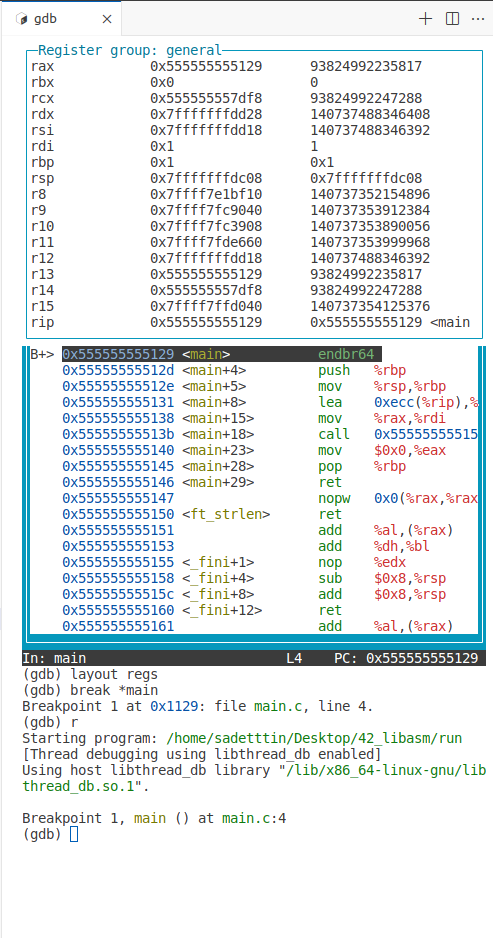
\includegraphics[width=0.55\textwidth]{gdb_assembly.png}
    \caption{Debugging Assembly Code with GDB}
    \label{fig:gdb_assembly}
\end{figure}

I used the figure \ref{fig:gdb_assembly} as a reference for debugging assembly code with GDB.

I run the following commands to debug the assembly code:
\begin{verbatim}
    make run
    gdb ./run
    (gdb) layout asm
    (gdb) layout regs
    (gdb) break *main
    (gdb) run
\end{verbatim}

\section{Tricks}

\subsection{argument passing in x64 Intel}
\begin{figure}[H]
    \centering
    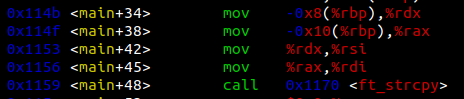
\includegraphics[width=0.8\textwidth]{trick.png}
    \caption{Argument passing for ft\_strcpy}
    \label{fig:trick}
\end{figure}

I noticed that when compiled with gcc (gcc main.c + libasm.a, libasm.a was compiled using nasm already) the first argument is passed in both rdx and rsi registers, and the second argument is passed in both rdi and rsi registers. I used the advantage this trick in my implementation by moving a register value and then substraction with fixed valued register and ta da.

\subsection{debuggin malloc}
\begin{figure}[H]
    \centering
    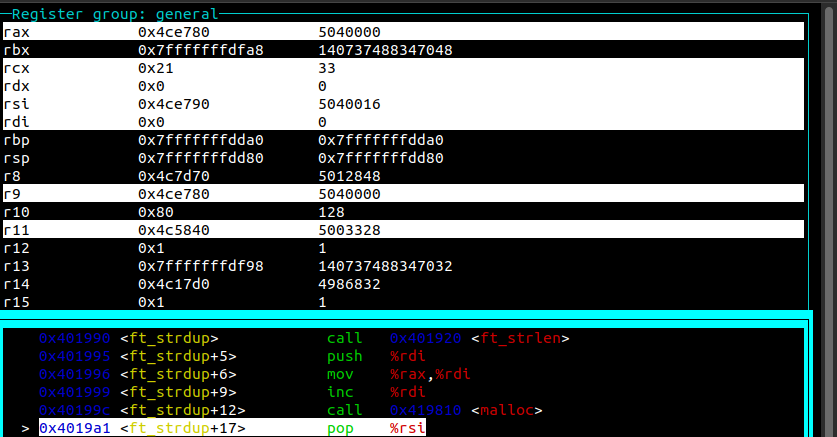
\includegraphics[width=0.8\textwidth]{regs_after_malloc.png}
    \caption{Registers affected by malloc}
    \label{fig:reg_malloc}
\end{figure}

\subsection{leave instruction}
\begin{figure}[H]
    \centering
    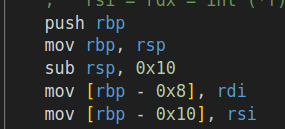
\includegraphics[width=0.8\textwidth]{leave.png}
    \caption{Leave instruction reverses this}
    \label{fig:leave}
\end{figure}

I used the leave instruction in the end of the function to reverse the stored up memory. The stored up memory is allocated for the local variables in the function as seen in the figure \ref{fig:leave}.

\subsection{offset calculation}
\begin{figure}[H]
    \centering
    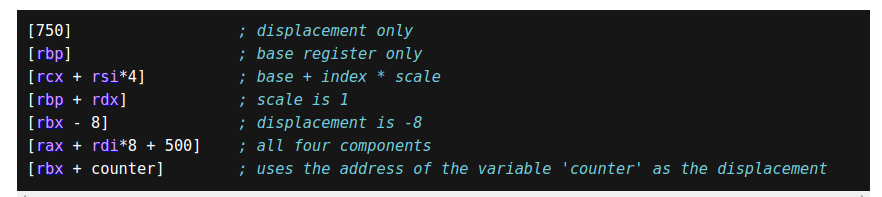
\includegraphics[width=0.8\textwidth]{offset.png}
    \caption{Offset calculation}
    \label{fig:offset}
\end{figure}

\end{document}